\documentclass[11pt,a4paper]{article}
\usepackage[utf8]{inputenc}
\usepackage[T1]{fontenc}
\usepackage{amsmath,amssymb}
\usepackage{booktabs}
\usepackage{longtable}
\usepackage{graphicx}
\usepackage[round,authoryear]{natbib}
\usepackage{hyperref}
\usepackage[margin=22mm]{geometry}
\usepackage{array}
\usepackage{xcolor}

\hypersetup{colorlinks=true,linkcolor=blue!60!black,citecolor=green!50!black,urlcolor=blue!70!black}
\setlength{\parskip}{0.45em}
\setlength{\parindent}{0pt}
\sloppy

\title{Novelty Assessment:\\
       AutoPos --- 3D Anchor Self-Calibration from Inter-Anchor Ranging Alone\\[5pt]
       \large System-Paper Positioning and Prior-Art Delineation}
\author{Zekai Xiao}
\date{June 2026}

\begin{document}
\maketitle

\section{One-Sentence Thesis}

AutoPos is, to our knowledge, the first UWB anchor self-calibration system that recovers full
\emph{3D} anchor coordinates jointly with per-device antenna delays from \emph{inter-anchor ranging
alone} --- with no external sensor (no LiDAR/SLAM/VIO/ultrasound), no mobile survey platform, and no
manually surveyed reference positions --- and that validates the result against optical ground
truth, reporting both the accuracy it reaches and the systematic vertical bias it does not remove.
The novelty is a \emph{deployment capability and its honest characterization}, not a new estimator:
the individual numerical components are established; what is new is their integration for the
inter-anchor-only 3D regime that prior work explicitly avoids, together with ground-truth-free
quality diagnostics usable at deployment time.

\section{Motivation: the Accuracy Ceiling and the Calibration Bottleneck}

The systematic review of 37 UWB$+$IMU motion-tracking systems by \citet{yogesh_2023} documents that
even the \emph{best} reported accuracy is only $\sim$5~cm: only $\sim$19\% of the systems reach
$\sim$10~cm even under ideal line-of-sight with optically surveyed anchors, the majority report
$10$--$80$~cm, and several exceed $1$~m --- all well short of the $\sim$1~cm that the review derives
from matching optical motion capture, the accuracy ``gold standard'' it considers clinically relevant. Only \emph{5 of the 37 systems attempt 3D positioning at all}; the other 32
operate purely in 2D, avoiding the vertical axis. The review singles out systematic UWB ranging error
as the dominant bottleneck, and its largest component is per-device antenna delay --- a constant
ranging bias of $\sim$150~mm per node \citep{shah_2021,sang_2019}, an order of magnitude above the
transceiver's random noise. The follow-up \citep{yogesh_2024} finds that none of the reviewed
systems even apply the manufacturer's recommended delay-calibration procedure --- let alone model
the delay inside their estimation pipeline --- and reports that even \emph{after} that procedure a
$\sim$3--4~cm systematic ranging residual remains.

The systems that do reach high accuracy do so only by importing infrastructure that is unavailable
out of the lab: angle-of-arrival base stations and surveyed anchor coordinates
\citep{zihajehzadeh_2017}, or dedicated
procedures requiring known reference positions \citep{kok_2015}. This is a \emph{circular
dependency}: accurate UWB positioning needs accurately known anchor coordinates, but obtaining those
coordinates needs an optical system or surveyed references --- precisely what is missing in
ambulatory, clinical, and field deployments. Anchor self-calibration is the route out of that
circle, and the gap AutoPos targets is that no existing self-calibration method closes it in 3D from
inter-anchor ranging alone on validated commodity hardware (Section~3).

\textbf{Why this system, and why $4{+}4$: the vertical axis has no shortcut.} The target application
is body-worn motion capture, which sharpens the requirement in a way that drone or robot UWB does
not. A hovering platform can resolve its height with an onboard downward range sensor (ultrasound,
time-of-flight) or fuse a barometer \citep{xiang_2025_uav}; a body-worn tag cannot --- an IMU gives only drifting relative
vertical displacement, and a barometer only coarse, drifting absolute height, neither adequate for
centimetre-level limb tracking. The \emph{only} drift-free, centimetre-level absolute vertical
reference available to a body-worn tag is the UWB geometry itself. The vertical must therefore be
carried by pure UWB, which is exactly why the array needs vertical geometric diversity (the balanced
$4{+}4$ two layers) rather than four coplanar anchors for the horizontal plus a height sensor on the tag.
This is also why what we term the \emph{delay--layout coupling} surfaced here at all: forcing UWB to
recover its weakest axis (the vertical) is precisely where a common-mode range bias aliases most
strongly, so a system required to obtain $Z$ from ranging alone is the one that exposes the coupling.
We name and stake the effect here; the companion paper (Paper~B) supplies its identifiability analysis.

\section{The Gap: A Narrow but Genuinely Unoccupied Combination}

UWB self-calibration splits cleanly into two clusters (Table~\ref{tab:cluster}), echoing the
two-cluster structure of the AutoPos concept's prior-art survey. The \emph{inter-anchor-only}
cluster is restricted to coplanar/2D deployments or requires a few manually surveyed reference
anchors; the \emph{3D} cluster achieves height observability only by adding an external sensor
(LiDAR, SLAM, or visual-inertial odometry) or a mobile platform that traverses the space ---
effectively replacing manual surveying with a robot-assisted survey. The combination ``3D $+$
inter-anchor ranging only $+$ joint antenna-delay $+$ no known reference'' is \emph{unoccupied as a
whole}, though every individual axis is occupied --- we say so explicitly to avoid an axis-stacked
``first.'' Joint anchor-plus-delay estimation already exists (\citealp{shah_2022};
\citealp{piavanini_2022}; \citealp{de_preter_2019}); 3D inter-anchor-only self-calibration without a
known reference exists in simulation (\citealp{pereira_2021}) and, via a \emph{mobile} platform on
hardware (\citealp{batstone_2017}). What is new is the \emph{conjunction} on commodity static
hardware with optical ground-truth validation, not any one ingredient. The conjunction is genuinely
hard, and the field documented it as such and stepped \emph{around} it rather than through it:
\citet{de_preter_2019} call the 3D calibration ``very ill-conditioned'' for similar tag/anchor heights
and restrict to 2D with tape-measured heights; \citet{corbalan_2023} report vertical resolution
``generally poor due to the low spread of anchors along that axis'' and recommend measuring height
independently; and commercial RTLS deployments that raise a few anchors to recover the vertical
\emph{survey} those raised positions rather than self-calibrate them. Each of these resolves the
vertical by importing a measured height --- the manual step AutoPos removes. AutoPos enters the regime
deliberately and reports what actually happens when the vertical is left to ranging alone --- which is
where the companion paper's delay finding emerges.

\begin{table}[h]
\centering
\setlength{\tabcolsep}{5pt}
\renewcommand{\arraystretch}{1.18}
\resizebox{\textwidth}{!}{%
\begin{tabular}{@{}lccccc@{}}
\toprule
Method & 3D & Inter-anchor only & Delay est. & No known ref. & GT-validated \\
\midrule
PANS auto-pos.\ \citep{decawave_2019}      & no & yes & no & yes & --- \\
Ridolfi 2021 \citep{ridolfi_2021}          & no (2D) & yes & no & yes & 2D \\
Piavanini 2022 \citep{piavanini_2022}      & no (2D) & yes & yes & yes & 2D \\
Corbalan 2023 \citep{corbalan_2023}        & no (2D) & yes & no & \textbf{no} & yes (2D) \\
De Preter 2019 \citep{de_preter_2019}      & no (2D) & \textbf{no} (mobile tag) & yes & \textbf{no} & RTK-GPS (2D) \\
Kok 2015 \citep{kok_2015}                  & yes & \textbf{no} & clock only & \textbf{no} & yes \\
Shah 2022 \citep{shah_2022}                & yes & \textbf{no} & yes & \textbf{no} & yes \\
Pereira 2021 \citep{pereira_2021}          & yes & yes & no & yes & sim.\ only \\
Batstone 2017 \citep{batstone_2017}        & yes & \textbf{no} (mobile tag) & no & yes & real-hw \\
Nguyen 2025 \citep{nguyen_2025}            & yes & \textbf{no} (SLAM) & yes & yes & SLAM-dep. \\
Yuan 2024 \citep{yuan_2024}                & yes & \textbf{no} (LiDAR) & implicit & yes & LiDAR-dep. \\
Liu \& Cao 2025 \citep{liu_2025}           & yes & \textbf{no} (LiDAR) & implicit & yes & LiDAR-dep. \\
Delama 2025 \citep{delama_2025}            & yes & \textbf{no} (VIO) & implicit & yes & VIO-dep. \\
\textbf{AutoPos (this work)}               & \textbf{yes} & \textbf{yes} & \textbf{yes} & \textbf{yes} & \textbf{Vicon} \\
\bottomrule
\end{tabular}}
\caption{Anchor self-calibration prior art. AutoPos occupies the otherwise-empty intersection of
3D, inter-anchor-ranging-only, joint antenna-delay estimation, and no known reference, validated
against optical ground truth. ``GT-validated'' = evaluated against an independent ground-truth
positioning system. ``Implicit'' delay = bias absorbed in optimization rather than explicitly
separated.}
\label{tab:cluster}
\end{table}

\section{What We Contribute}

\textbf{(1) The capability --- and a reference point for later work.} The headline result is a
pure-UWB, self-calibrated vertical of ${\approx}62$~mm median absolute error (vs Vicon), against a Fisher-predicted ${\approx}63$~mm
inter-anchor vertical CRLB for $4{+}4$, from inter-anchor ranging alone --- a reference point that later
reference-free pure-UWB vertical self-calibration in this deployment regime can be measured against. It is produced by a
complete, real-hardware pipeline (8$\times$ DWM1001C, two elevation levels) that takes bidirectional
SS-TWR inter-anchor ranging to a 3D anchor layout with per-device antenna delays, using only commodity
single-antenna TWR modules --- two orders of magnitude cheaper
than the AoA base stations \citep{zihajehzadeh_2017} or optical systems prior high-accuracy work
relies on, and without the mobile sensor rigs the 3D self-calibration cluster requires. The deployed
custom SS-TWR firmware applies a single generic antenna-delay default (the vendor example value,
16436 device units) identically to every node, with no per-device hardware calibration; the
per-device delays the solver estimates are precisely the residuals this generic default leaves in the
ranging. Calibration is thus pushed entirely into the AutoPos software solve --- which is the
realistic out-of-the-box deployment condition, and the physical reason a delay term is needed at all.

\textbf{(2) The geometry that makes the cell enterable.} A balanced two-layer $4{+}4$ non-coplanar
array. Non-coplanarity for 3D is itself known; our claim is narrower and is a statement about the
\emph{self-calibration} regime specifically: under reference-free inter-anchor self-calibration --- and with all eight anchors participating in the ranging --- a
\emph{balanced} upper layer is what restores well-conditioned vertical \emph{geometry}, whereas an
asymmetric raise (e.g.\ one or two anchors lifted) leaves the vertical ill-conditioned. Deployed
systems that raise a few anchors do not hit this wall --- but only because they \emph{survey} the
raised positions rather than self-calibrate them, sidestepping the conditioning by importing the very
measurement AutoPos removes. We quantify this with a self-calibration Fisher analysis (Figure~\ref{fig:vobs}): for a single
coplanar layer the inter-anchor vertical Cram\'{e}r--Rao bound is \emph{exactly singular}
($\partial r/\partial z=0$). A single raised anchor formally unlocks the vertical but leaves it
badly conditioned (mean vertical CRLB $\sim$161~mm, worst-anchor $\sim$226~mm at $4{+}1$); adding
upper anchors improves it monotonically. Crucially the \emph{mean} bound saturates early
($\sim$81~mm at $4{+}2$, $\sim$63~mm at $4{+}4$), so an average alone would suggest stopping at two
--- but the \emph{worst-conditioned} anchor keeps falling ($226\!\to\!134\!\to\!122\!\to\!93$~mm
across $4{+}1,\,4{+}2,\,4{+}3,\,4{+}4$). The balanced $4{+}4$ is therefore the smallest array that
brings \emph{every} anchor's vertical to the production floor on average ($\sim$63~mm RMS bound, the same order as
the deployed median vertical error of ${\approx}62$~mm) and to no worse than $\sim$93~mm: the choice over an asymmetric
$4{+}k$ raise is a worst-case-uniformity argument, not an observability one. At fixed anchor count a
\emph{balanced} (diagonal) pair beats a \emph{clustered} (adjacent) pair by $1.24\times$, confirming
that it is the balance, not merely the count, that conditions the vertical.

\begin{figure}[h]
\centering
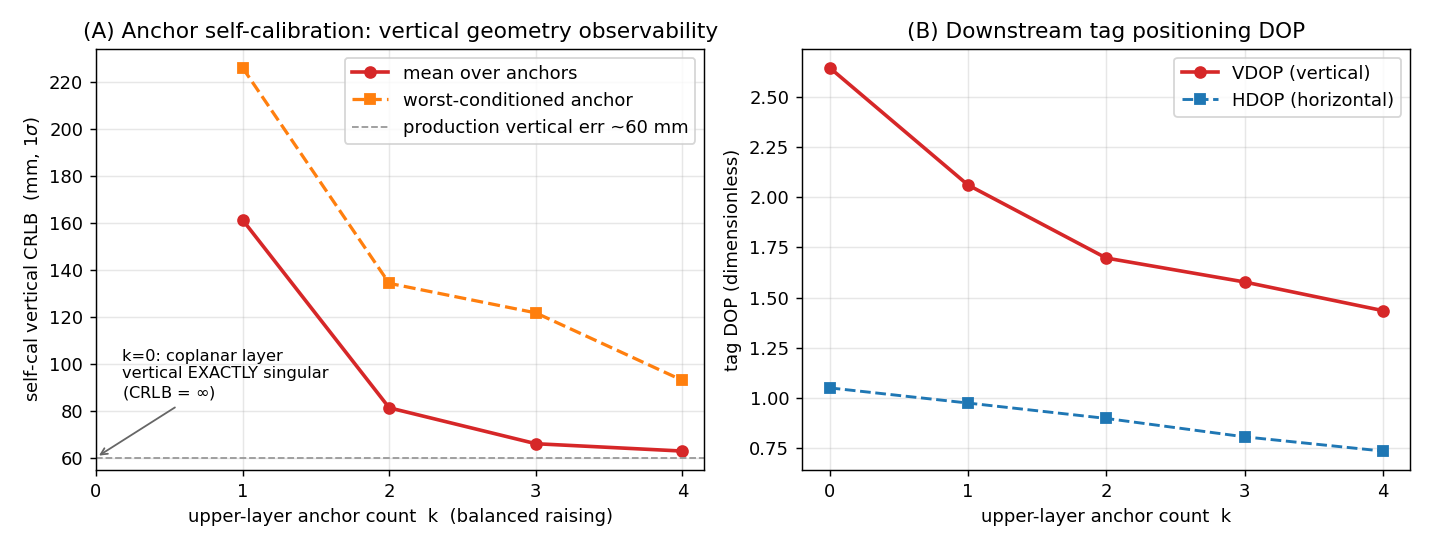
\includegraphics[width=0.92\textwidth]{literature_search/vertical_observability_4plus4.png}
\caption{Vertical observability vs.\ upper-layer anchor count $k$ (balanced raising).
\textbf{(A)} Anchor self-calibration vertical CRLB from inter-anchor ranging: singular for a
coplanar layer ($k{=}0$). The \emph{mean} bound (circles) saturates near the $\sim$63~mm production
vertical error by $k{=}2$, but the \emph{worst-conditioned} anchor (squares) keeps improving to
$k{=}4$ ($226\!\to\!134\!\to\!122\!\to\!93$~mm), so the balanced $4{+}4$ is the smallest array with
\emph{uniformly} well-conditioned vertical geometry --- the case against an asymmetric $4{+}k$ raise.
\textbf{(B)} Downstream tag-localization DOP for the same idealized balanced array: vertical
(VDOP) improves monotonically with $k$ but remains the worse-determined axis throughout
(VDOP $>$ HDOP). The deployment geometry's measured vertical DOP penalty is reported in the
companion mechanism paper.}
\label{fig:vobs}
\end{figure}

\emph{Why eight anchors, not more.} The anchor count is set by a system constraint, not chosen for
convenience --- which answers the natural ``why not $8{+}8$ for better geometry?'' To keep
\emph{moving} body-worn tags consistent, the ranging uses a \textbf{broadcast} scheme so that all
anchors observe the same transmission instant, eliminating the motion-induced error that sequential
per-anchor ranging accumulates as the tag moves; and the system is dimensioned for \textbf{10~Hz
updates on up to 10 simultaneous tags}. That throughput and motion-coherence budget caps how many
anchors can be ranged per cycle, so the balanced $4{+}4$ is the \emph{minimum} two-layer configuration
that still reaches the vertical-observability floor (Figure~\ref{fig:vobs}) within the budget --- a
denser array such as $8{+}8$ would either break the 10~Hz$\times$10-tag throughput or reintroduce
motion error. The claim is therefore not ``use more anchors for better geometry'' but ``reach
vertical observability with the fewest anchors a real-time multi-tag broadcast system can afford.''

\textbf{(3) Two deployment diagnostics that need no ground truth.} Optical ground truth is exactly
what is unavailable at deployment, so we identify two checks that flag a bad calibration using only
the UWB data itself.

\begin{itemize}
\item \emph{Ranging residual is a misleading quality signal.} With only four anchors in a fix --- three
      position unknowns and one redundant measurement --- the solver can fit the four distances
      almost perfectly even when the recovered position is wrong, so the configuration with the
      \emph{lowest} residual can have the \emph{worst} position. In our data the lowest-residual
      variant (11.5~mm) gives the worst positioning ($\sim$169~mm), while the best positioner
      (49~mm) has a slightly \emph{higher} residual (12.9~mm). The practical lesson: do not trust
      ranging residual as a calibration-quality score unless there are redundant anchors
      ($\geq 6$).
\item \emph{Dispersion across dynamic anchor selection exposes hidden bias.} When all~8 anchors are
      used for every fix, any systematic calibration error appears as a constant offset and all
      solver variants look equally good ($\sim$28--33~mm). The differences only appear when the tag
      selects a \emph{different} 4-anchor subset per fix: a well-calibrated layout still yields
      consistent positions across subsets, whereas a biased layout yields scattered ones. The
      spread across subsets is therefore a calibration-quality indicator that a fixed anchor set
      would hide --- and, crucially, it needs no ground truth.
\end{itemize}

\textbf{(4) Honest validation.} We convert the system from a repeatability claim to a ground-truth
claim using optical motion capture, and report both the accuracy and the limit (next section).

\section{What We Are \emph{Not} Claiming (and the honest limits)}

\begin{itemize}
\item \textbf{Not a new estimator.} SDP/MDS initialization, Tukey-bisquare IRLS, MAD/MVUE fusion, and
      alternating joint antenna-delay estimation are individually established. Joint estimation of
      anchor coordinates and per-anchor range bias from ranging is itself prior art
      (\citealp{de_preter_2019}; \citealp{piavanini_2022}; \citealp{shah_2022}). Closest on the
      bias-estimation side is \citet{yogesh_2024}, which estimates per-node additive range bias in a
      fully-connected UWB \emph{swarm} validated against optical ground truth --- but with the node
      positions \emph{known} (from the optical system) and an explicitly pure-additive bias model, so
      it calibrates bias rather than self-calibrating geometry, and requires the very external
      reference AutoPos removes. The contribution here is the integration for the 3D inter-anchor-only,
      reference-free regime and the ground-truth characterization, not the algorithms.
\item \textbf{The antenna delays are estimated and empirically useful, not yet independently
      validated as physical delays.} Their correctness is currently inferred only through downstream
      positioning and scale, so we report them as estimated-and-useful rather than ``recovered.'' A
      factory-OTP cross-check was attempted but cannot serve this purpose: across all nine modules the
      DW1000 OTP stores only a near-uniform lot-level antenna-delay value with no per-device antenna
      calibration, so it does not supply the per-device delays the solver estimates --- a finding that
      itself matters for the companion paper, where it is reported in full.
\item \textbf{Consistency is not accuracy.} The preliminary headline numbers (positioning standard
      deviation of order $5$~cm 3D / $4$~cm vertical) measure repeatability of repeated fixes, not
      absolute error. Against optical ground truth the absolute error is larger, and only the
      ground-truth-validated numbers are reported as accuracy.
\item \textbf{The $4{+}4$ geometry is necessary, not sufficient, for the vertical.} It completes the
      vertical \emph{geometric} observability, but a systematic vertical bias remains after it ---
      because that residual is not a geometry deficit but a \emph{tag-side} delay aliasing into the vertical. The Fisher
      analysis makes this concrete: the inter-anchor vertical CRLB saturates near $63$~mm for $4{+}4$,
      at the level of the ${\approx}62$~mm deployed median vertical error --- a bound on the \emph{anchor}
      geometry's vertical contribution, not on the tag positioning error, but their closeness indicates
      the geometry is near its floor, so the residual vertical bias is consistent with a tag-side delay
      alias rather than a geometry deficit. This is the single most important honest caveat, and it is
      the tag-side face of the delay--layout coupling the companion paper analyzes, distinct from that
      paper's \emph{headline} anchor-side delay$\leftrightarrow$scale result.
\item \textbf{We do not claim general superiority of self-calibration over surveying} for
      applications demanding the highest achievable accuracy; we claim a favorable
      effort/accuracy/cost trade-off for rapid, equipment-free 3D deployment.
\end{itemize}

\section{Accuracy by Axis, and the Pure-UWB Vertical}

We report two distinct quantities and never conflate them: \emph{repeatability} (standard deviation
of repeated static fixes, the headline $\sim$5~cm number) and \emph{absolute accuracy} (error against
Vicon, which is what the literature reports). The comparison to the landscape uses the absolute
numbers.

\textbf{Horizontal (X--Y plane).} Repeatability $\sim$27~mm; absolute $\sim$37~mm (median vs Vicon). This sits in the
same band as the horizontal accuracy of the best fusion systems ($\sim$30--40~mm per axis). The
horizontal is the easy axis for everyone; we neither lead nor lag here.

\textbf{Vertical --- the standout.} Repeatability $\sim$41~mm; absolute $\sim$62~mm (median vs Vicon), from \emph{pure
UWB} with self-calibrated anchors, no IMU fusion, no AoA hardware, no surveyed anchors, and no
external height sensor. This is the axis the field cannot get cheaply: 32 of the 37 reviewed systems
avoid it (2D); the systems that do resolve it import a crutch a body-worn tag cannot use --- AoA base
stations plus biomechanical constraints plus OptiTrack \citep{zihajehzadeh_2017}, or surveyed anchors
plus IMU fusion. The pure-UWB vertical here lands in the band that
others reach only with external help. \textbf{The defensible claim is not ``smallest vertical
number'' but ``a usable vertical recovered from UWB alone, under the body-worn constraint that rules
out every external height aid''} --- which is precisely why the balanced $4{+}4$ array exists.

\textbf{3D total.} Repeatability $\sim$50~mm ($\sim$28~mm when all eight anchors are visible online);
absolute $\sim$73~mm median (P95 ${\approx}172$~mm, RMSE ${\approx}110$~mm). This sits in the upper range of the reviewed systems
($10$--$80$~cm) and within reach of the best ($\sim$48~mm 3D RMSE), though we do \emph{not} claim it
is the single smallest absolute number: the best reviewed result ($\sim$48~mm, a 24~s walk with
surveyed anchors and IMU fusion) still edges it. The ${\approx}73$~mm median further benefits, in part,
from the self-calibrated production layout's expanded scale compensating an uncorrected tag-side
delay: with the tag-side delay left at zero, the clean metric-corrected layout gives a larger
${\approx}110$~mm median (the mechanism and its in-environment control are analyzed in the companion paper).

\textbf{Honest caveat on the comparison.} The reviewed systems are UWB$+$IMU \emph{fusion} tracking a
\emph{moving} tag; AutoPos is UWB-only positioning of a \emph{static} tag. Fusion and IMU help them;
the static setting helps us. So the correct statement is that AutoPos reaches the same accuracy band
\emph{UWB-only and self-calibrated, with a resolved vertical}, not that it beats fusion systems. The
absolute vertical is referenced to the optical marker, so a fixed marker-to-antenna-phase-centre offset
would shift this absolute value (the companion paper's phase-center sensitivity check finds the layout
ranking robust to marker offsets beyond 10~mm).

\textbf{Anchor visibility.} Visibility was high across the 24-position static campaign: at every position
$92.2\%$ of frames ranged to all eight anchors and $99.9\%$ to at least seven (per-position median
$8/8$; link-level success $99.0\%$). The residual single-anchor dropout was dominated by
one anchor (${\sim}4.4\%$ of its frames; the others below $2\%$). Because a seven-of-eight fix remains
non-coplanar and over-determined, the vertical conditioning is preserved in $99.9\%$ of frames, so the
reported medians are effectively whole-array fixes rather than a full-visibility subset.

\textbf{Reproducibility scope --- full-array participation is part of the method.} The positioning
numbers above are obtained at the system's designed operating point, where \emph{every fix draws on
all eight anchors} of the two-layer array. This is constitutive, not a favourable selection --- and it
is the eight-anchor participation, not the ranging protocol, that conditions the vertical: for a static
fix a sequential and a broadcast acquisition give the same ranges. A reproduction that admits fixes
from \emph{fewer} anchors (e.g.\ a four-anchor subset) raises the vertical CRLB sharply, while collapsing
the array to a single coplanar layer returns the vertical to the ill-conditioned
$\partial r/\partial z \to 0$ regime the Fisher analysis proves exactly singular; neither recovers these
numbers. The graceful, layer-asymmetric degradation under partial anchor dropout (losing an
\emph{upper} versus a \emph{lower} anchor is not equivalent) is characterised by the stratified
keep-$k$ analysis in the full system evaluation.

\section{Relationship to the Companion Mechanism Paper}

The companion mechanism paper (Paper~B) is the natural home for the finding that this system
surfaces: that the residual vertical error is the per-tag projection of a common-mode range bias ---
the UWB analogue of the GPS receiver-clock/altitude coupling --- which no amount of added geometric
diversity removes, only an explicit tag-delay correction (demonstrated there by an active vertical-injection control that produced no dose-response). Keeping the two
separate avoids cannibalizing the higher-tier mechanism paper with the systems paper, and lets the
mechanism paper cite this validated system as the substrate for its analysis. Paper~A establishes
priority on the deployment capability and the balanced $4{+}4$ geometry; Paper~B establishes
priority on the delay--layout coupling --- headlined by the anchor-side delay$\leftrightarrow$scale
identifiability analysis and the falsification protocol, with the tag-side vertical aliasing above as
the strand that bears on this system's residual limit.

\section*{Draft Front-Matter (Abstract, Keywords, Key Claim)}

\textbf{Abstract (draft).}
\begin{quote}\small
Anchor-based ultra-wideband (UWB) positioning requires accurately known anchor coordinates, yet for
body-worn motion capture the vertical axis has no shortcut: unlike a hovering platform, a body-worn
tag cannot carry a downward range sensor or usefully fuse a barometer, so a drift-free,
centimetre-level vertical reference can come only from the UWB geometry itself. We present a
reference-free 3D anchor self-calibration that recovers anchor coordinates and per-device antenna
delays from inter-anchor two-way ranging alone --- no external sensor, no mobile survey platform, no
surveyed reference positions --- on commodity (DWM1001C) hardware, validated against optical (Vicon)
ground truth. The enabling element is a balanced two-layer ($4{+}4$) anchor array: via a
Fisher/Cram\'{e}r--Rao analysis we show a single coplanar layer leaves the vertical exactly
unobservable ($\partial r/\partial z = 0$), that raising anchors unlocks it, and that the balanced
$4{+}4$ array reaches a vertical CRLB floor of ${\approx}63$~mm, with \emph{balance} --- not merely
anchor count --- conditioning the vertical; the eight-anchor count itself follows from a real-time
broadcast protocol dimensioned for 10~Hz on up to 10 simultaneous tags. Reporting by axis and
separating repeatability from absolute accuracy, the system attains ${\approx}5$~cm 3D / ${\approx}4$~cm
vertical repeatability and ${\approx}7$~cm 3D / ${\approx}6$~cm absolute (vs Vicon) --- a pure-UWB
vertical where most comparable systems avoid the axis or reach it only with angle-of-arrival,
biomechanical, or surveyed-anchor aids. The $4{+}4$ geometry is necessary but not sufficient: a residual systematic vertical
bias remains, attributed to a tag-side delay aliasing into the vertical (companion paper). To our knowledge this is
the first demonstration that the \emph{vertical} axis of a UWB anchor array can be self-calibrated to
the centimetre level --- ${\approx}62$~mm median absolute against optical ground truth, with a Fisher-predicted ${\approx}63$~mm
inter-anchor vertical CRLB for $4{+}4$ --- from inter-anchor ranging alone on commodity single-antenna
modules, with the delay coupling that bounds it identified and quantified.
\end{quote}

\textbf{Keywords.} ultra-wideband (UWB); anchor self-calibration; anchor auto-positioning;
reference-free / infrastructure-free localization; inter-anchor two-way ranging (TWR); two-layer
anchor array; vertical observability; 3D positioning; antenna-delay calibration; body-worn / wearable
motion capture; Cram\'{e}r--Rao bound; dilution of precision.

\textbf{Key claim.} \emph{``A balanced two-layer
($4{+}4$) anchor array renders the vertical \emph{well-conditioned} for reference-free, inter-anchor-only 3D UWB
self-calibration --- a single coplanar layer is exactly singular ($\partial r/\partial z = 0$) and a single raised anchor only weakly unlocks it, while
the balanced $4{+}4$ reaches a ${\approx}63$~mm vertical Cram\'{e}r--Rao floor --- enabling a pure-UWB
vertical without any external height aid.''}

\begin{thebibliography}{99}

\bibitem[Batstone et~al.(2017)]{batstone_2017} Batstone, K., Oskarsson, M. and \AA{}str\"om, K.,
2017. Towards real-time time-of-arrival self-calibration using ultra-wideband anchors. In:
\emph{International Conference on Indoor Positioning and Indoor Navigation (IPIN)}, pp.1--8.

\bibitem[Corbalan et~al.(2023)]{corbalan_2023} Corbalan, P., Picco, G.P., Coors, M. and Jain, V.,
2023. Self-localization of ultra-wideband anchors: From theory to practice. \emph{IEEE Access}, 11,
pp.29711--29725.

\bibitem[De Preter et~al.(2019)]{de_preter_2019} De Preter, A., Goysens, G., Anthonis, J., Swevers,
J. and Pipeleers, G., 2019. Range bias modeling and autocalibration of a UWB positioning system. In:
\emph{International Conference on Indoor Positioning and Indoor Navigation (IPIN)}, pp.1--8.

\bibitem[Decawave/Qorvo(2019)]{decawave_2019} Decawave Ltd., 2019. \emph{MDEK1001 Kit User Manual}
(DWM1001 module development and evaluation kit; PANS auto-positioning). Version 1.2.

\bibitem[Delama et~al.(2025)]{delama_2025} Delama, G., Borowski, I., Jung, R. and Weiss, S., 2025.
Real-time initialization of unknown anchors for UWB-aided navigation. In: \emph{IEEE/RSJ
International Conference on Intelligent Robots and Systems (IROS)}. arXiv:2506.15518.

\bibitem[Kok et~al.(2015)]{kok_2015} Kok, M., Hol, J.D. and Sch\"on, T.B., 2015. Indoor positioning
using ultrawideband and inertial measurements. \emph{IEEE Transactions on Vehicular Technology},
64(4), pp.1293--1303.

\bibitem[Nguyen et~al.(2025)]{nguyen_2025} Nguyen, T.-D., Nguyen, T.-M. and Nguyen, V.-H., 2025.
Coordinate-consistent localization via continuous-time calibration and fusion of UWB and SLAM
observations. \emph{arXiv preprint} arXiv:2510.05992.

\bibitem[Liu and Cao(2025)]{liu_2025} Liu, X. and Cao, M., 2025. Robust simultaneous UWB-anchor
calibration and robot localization for emergency situations. \emph{arXiv preprint} arXiv:2503.22272.

\bibitem[Pereira(2021)]{pereira_2021} Pereira, J., 2021. \emph{Anchor self-calibrating schemes for
UWB based indoor localization}. M.Sc.\ thesis, Rochester Institute of Technology.

\bibitem[Piavanini et~al.(2022)]{piavanini_2022} Piavanini, M., Barbieri, L., Brambilla, M., Cerutti,
M., Ercoli, S., Agili, A. and Nicoli, M., 2022. A self-calibrating localization solution for sport
applications with UWB technology. \emph{Sensors}, 22(23), 9363.

\bibitem[Ridolfi et~al.(2021)]{ridolfi_2021} Ridolfi, M., Fontaine, J., Van Herbruggen, B., Joseph,
W., Hoebeke, J. and De Poorter, E., 2021. UWB anchor nodes self-calibration in NLOS conditions: A
machine learning and adaptive PHY error correction approach. \emph{Wireless Networks}, 27,
pp.3007--3023.

\bibitem[Sang et~al.(2019)]{sang_2019} Sang, C.L., Adams, M., H\"ormann, T., Hesse, M., Porrmann, M. and R\"uckert, U., 2019. Numerical and
experimental evaluation of error estimation for two-way ranging methods. \emph{Sensors}, 19(3), 616.

\bibitem[Shah et~al.(2021)]{shah_2021} Shah, S., Chaiwong, K., Kovavisaruch, L., Kaemarungsi, K. and
Demeechai, T., 2021. Antenna delay calibration of UWB nodes. \emph{IEEE Access}, 9,
pp.63294--63305.

\bibitem[Shah et~al.(2022)]{shah_2022} Shah, S., Kovavisaruch, L., Kaemarungsi, K. and
Demeechai, T., 2022. Node calibration in UWB-based RTLSs using multiple simultaneous ranging.
\emph{Sensors}, 22(3), 864.

\bibitem[Xiang et~al.(2025)]{xiang_2025_uav} Xiang, Z., Chen, L., Wu, Q., Yang, J., Dai, X. and Xie, X.,
2025. An improved UWB indoor positioning approach for UAVs based on the dual-anchor model.
\emph{Sensors}, 25(4), 1052.

\bibitem[Yogesh et~al.(2023)]{yogesh_2023} Yogesh, V., Buurke, J.H., Veltink, P.H. and Baten,
C.T.M., 2023. Integrated UWB/MIMU sensor system for position estimation towards an accurate analysis
of human movement: A technical review. \emph{Sensors}, 23(16), 7277.

\bibitem[Yogesh et~al.(2024)]{yogesh_2024} Yogesh, V., Grevinga, L., Voort, C., Buurke, J.H.,
Veltink, P.H. and Baten, C.T.M., 2024. Novel calibration method for improved UWB sensor distance
measurement in the context of application for 3D analysis of human movement. \emph{Engineering
Science and Technology, an International Journal}, 58, 101844.

\bibitem[Yuan et~al.(2024)]{yuan_2024} Yuan, S., Lou, B., Nguyen, T.-M., Yin, P., Cao, M., Xu, X., Li, J., Xu, J., Chen, S. and Xie, L.,
2024. Large-scale UWB anchor calibration and one-shot localization using Gaussian process.
\emph{arXiv preprint} arXiv:2412.16880.

\bibitem[Zihajehzadeh and Park(2017)]{zihajehzadeh_2017} Zihajehzadeh, S. and Park, E.J., 2017. A
novel biomechanical model-aided IMU/UWB fusion for magnetometer-free lower body motion capture.
\emph{IEEE Transactions on Systems, Man, and Cybernetics: Systems}, 47(6), pp.927--938.

\end{thebibliography}

\end{document}
